\documentclass[1p]{elsarticle_modified}
%\bibliographystyle{elsarticle-num}

%\usepackage[colorlinks]{hyperref}
%\usepackage{abbrmath_seonhwa} %\Abb, \Ascr, \Acal ,\Abf, \Afrak
\usepackage{amsfonts}
\usepackage{amssymb}
\usepackage{amsmath}
\usepackage{amsthm}
\usepackage{scalefnt}
\usepackage{amsbsy}
\usepackage{kotex}
\usepackage{caption}
\usepackage{subfig}
\usepackage{color}
\usepackage{graphicx}
\usepackage{xcolor} %% white, black, red, green, blue, cyan, magenta, yellow
\usepackage{float}
\usepackage{setspace}
\usepackage{hyperref}

\usepackage{tikz}
\usetikzlibrary{arrows}

\usepackage{multirow}
\usepackage{array} % fixed length table
\usepackage{hhline}

%%%%%%%%%%%%%%%%%%%%%
\makeatletter
\renewcommand*\env@matrix[1][\arraystretch]{%
	\edef\arraystretch{#1}%
	\hskip -\arraycolsep
	\let\@ifnextchar\new@ifnextchar
	\array{*\c@MaxMatrixCols c}}
\makeatother %https://tex.stackexchange.com/questions/14071/how-can-i-increase-the-line-spacing-in-a-matrix
%%%%%%%%%%%%%%%

\usepackage[normalem]{ulem}

\newcommand{\msout}[1]{\ifmmode\text{\sout{\ensuremath{#1}}}\else\sout{#1}\fi}
%SOURCE: \msout is \stkout macro in https://tex.stackexchange.com/questions/20609/strikeout-in-math-mode

\newcommand{\cancel}[1]{
	\ifmmode
	{\color{red}\msout{#1}}
	\else
	{\color{red}\sout{#1}}
	\fi
}

\newcommand{\add}[1]{
	{\color{blue}\uwave{#1}}
}

\newcommand{\replace}[2]{
	\ifmmode
	{\color{red}\msout{#1}}{\color{blue}\uwave{#2}}
	\else
	{\color{red}\sout{#1}}{\color{blue}\uwave{#2}}
	\fi
}

\newcommand{\Sol}{\mathcal{S}} %segment
\newcommand{\D}{D} %diagram
\newcommand{\A}{\mathcal{A}} %arc


%%%%%%%%%%%%%%%%%%%%%%%%%%%%%5 test

\def\sl{\operatorname{\textup{SL}}(2,\Cbb)}
\def\psl{\operatorname{\textup{PSL}}(2,\Cbb)}
\def\quan{\mkern 1mu \triangleright \mkern 1mu}

\theoremstyle{definition}
\newtheorem{thm}{Theorem}[section]
\newtheorem{prop}[thm]{Proposition}
\newtheorem{lem}[thm]{Lemma}
\newtheorem{ques}[thm]{Question}
\newtheorem{cor}[thm]{Corollary}
\newtheorem{defn}[thm]{Definition}
\newtheorem{exam}[thm]{Example}
\newtheorem{rmk}[thm]{Remark}
\newtheorem{alg}[thm]{Algorithm}

\newcommand{\I}{\sqrt{-1}}
\begin{document}

%\begin{frontmatter}
%
%\title{Boundary parabolic representations of knots up to 8 crossings}
%
%%% Group authors per affiliation:
%\author{Yunhi Cho} 
%\address{Department of Mathematics, University of Seoul, Seoul, Korea}
%\ead{yhcho@uos.ac.kr}
%
%
%\author{Seonhwa Kim} %\fnref{s_kim}}
%\address{Center for Geometry and Physics, Institute for Basic Science, Pohang, 37673, Korea}
%\ead{ryeona17@ibs.re.kr}
%
%\author{Hyuk Kim}
%\address{Department of Mathematical Sciences, Seoul National University, Seoul 08826, Korea}
%\ead{hyukkim@snu.ac.kr}
%
%\author{Seokbeom Yoon}
%\address{Department of Mathematical Sciences, Seoul National University, Seoul, 08826,  Korea}
%\ead{sbyoon15@snu.ac.kr}
%
%\begin{abstract}
%We find all boundary parabolic representation of knots up to 8 crossings.
%
%\end{abstract}
%\begin{keyword}
%    \MSC[2010] 57M25 
%\end{keyword}
%
%\end{frontmatter}

%\linenumbers
%\tableofcontents
%
\newcommand\colored[1]{\textcolor{white}{\rule[-0.35ex]{0.8em}{1.4ex}}\kern-0.8em\color{red} #1}%
%\newcommand\colored[1]{\textcolor{white}{ #1}\kern-2.17ex	\textcolor{white}{ #1}\kern-1.81ex	\textcolor{white}{ #1}\kern-2.15ex\color{red}#1	}

{\Large $\underline{12n_{0019}~(K12n_{0019})}$}

\setlength{\tabcolsep}{10pt}
\renewcommand{\arraystretch}{1.6}
\vspace{1cm}\begin{tabular}{m{100pt}>{\centering\arraybackslash}m{274pt}}
\multirow{5}{120pt}{
	\centering
	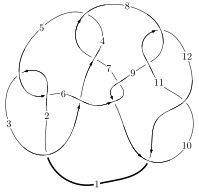
\includegraphics[width=112pt]{../../../GIT/diagram.site/Diagrams/png/2108_12n_0019.png}\\
\ \ \ A knot diagram\footnotemark}&
\allowdisplaybreaks
\textbf{Linearized knot diagam} \\
\cline{2-2}
 &
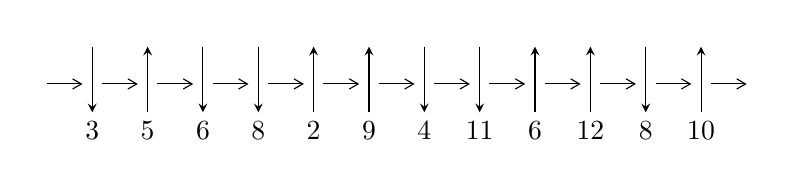
\begin{tikzpicture}[x=20pt, y=17pt]
	% nodes
	\node (C0) at (0, 0) {};
	\node (C1) at (1, 0) {};
	\node (C1U) at (1, +1) {};
	\node (C1D) at (1, -1) {3};

	\node (C2) at (2, 0) {};
	\node (C2U) at (2, +1) {};
	\node (C2D) at (2, -1) {5};

	\node (C3) at (3, 0) {};
	\node (C3U) at (3, +1) {};
	\node (C3D) at (3, -1) {6};

	\node (C4) at (4, 0) {};
	\node (C4U) at (4, +1) {};
	\node (C4D) at (4, -1) {8};

	\node (C5) at (5, 0) {};
	\node (C5U) at (5, +1) {};
	\node (C5D) at (5, -1) {2};

	\node (C6) at (6, 0) {};
	\node (C6U) at (6, +1) {};
	\node (C6D) at (6, -1) {9};

	\node (C7) at (7, 0) {};
	\node (C7U) at (7, +1) {};
	\node (C7D) at (7, -1) {4};

	\node (C8) at (8, 0) {};
	\node (C8U) at (8, +1) {};
	\node (C8D) at (8, -1) {11};

	\node (C9) at (9, 0) {};
	\node (C9U) at (9, +1) {};
	\node (C9D) at (9, -1) {6};

	\node (C10) at (10, 0) {};
	\node (C10U) at (10, +1) {};
	\node (C10D) at (10, -1) {12};

	\node (C11) at (11, 0) {};
	\node (C11U) at (11, +1) {};
	\node (C11D) at (11, -1) {8};

	\node (C12) at (12, 0) {};
	\node (C12U) at (12, +1) {};
	\node (C12D) at (12, -1) {10};
	\node (C13) at (13, 0) {};

	% arrows
	\draw[->,>={angle 60}]
	(C0) edge (C1) (C1) edge (C2) (C2) edge (C3) (C3) edge (C4) (C4) edge (C5) (C5) edge (C6) (C6) edge (C7) (C7) edge (C8) (C8) edge (C9) (C9) edge (C10) (C10) edge (C11) (C11) edge (C12) (C12) edge (C13) ;	\draw[->,>=stealth]
	(C1U) edge (C1D) (C2D) edge (C2U) (C3U) edge (C3D) (C4U) edge (C4D) (C5D) edge (C5U) (C6D) edge (C6U) (C7U) edge (C7D) (C8U) edge (C8D) (C9D) edge (C9U) (C10D) edge (C10U) (C11U) edge (C11D) (C12D) edge (C12U) ;
	\end{tikzpicture} \\
\hhline{~~} \\& 
\textbf{Solving Sequence} \\ \cline{2-2} 
 &
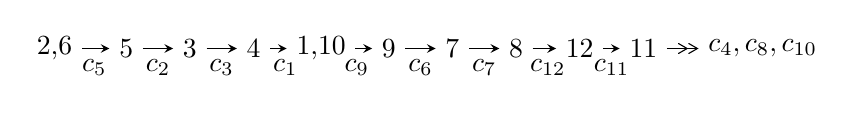
\begin{tikzpicture}[x=23pt, y=7pt]
	% node
	\node (A0) at (-1/8, 0) {2,6};
	\node (A1) at (1, 0) {5};
	\node (A2) at (2, 0) {3};
	\node (A3) at (3, 0) {4};
	\node (A4) at (65/16, 0) {1,10};
	\node (A5) at (41/8, 0) {9};
	\node (A6) at (49/8, 0) {7};
	\node (A7) at (57/8, 0) {8};
	\node (A8) at (65/8, 0) {12};
	\node (A9) at (73/8, 0) {11};
	\node (C1) at (1/2, -1) {$c_{5}$};
	\node (C2) at (3/2, -1) {$c_{2}$};
	\node (C3) at (5/2, -1) {$c_{3}$};
	\node (C4) at (7/2, -1) {$c_{1}$};
	\node (C5) at (37/8, -1) {$c_{9}$};
	\node (C6) at (45/8, -1) {$c_{6}$};
	\node (C7) at (53/8, -1) {$c_{7}$};
	\node (C8) at (61/8, -1) {$c_{12}$};
	\node (C9) at (69/8, -1) {$c_{11}$};
	\node (A10) at (11, 0) {$c_{4},c_{8},c_{10}$};

	% edge
	\draw[->,>=stealth]	
	(A0) edge (A1) (A1) edge (A2) (A2) edge (A3) (A3) edge (A4) (A4) edge (A5) (A5) edge (A6) (A6) edge (A7) (A7) edge (A8) (A8) edge (A9) ;
	\draw[->>,>={angle 60}]	
	(A9) edge (A10);
\end{tikzpicture} \\ 

\end{tabular} \\

\footnotetext{
The image of knot diagram is generated by the software ``\textbf{Draw programme}" developed by Andrew Bartholomew(\url{http://www.layer8.co.uk/maths/draw/index.htm\#Running-draw}), where we modified some parts for our purpose(\url{https://github.com/CATsTAILs/LinksPainter}).
}\phantom \\ \newline 
\centering \textbf{Ideals for irreducible components\footnotemark of $X_{\text{par}}$} 
 
\begin{align*}
I^u_{1}&=\langle 
222 u^{17}+1807 u^{16}+\cdots+536 b-1177,\;-19 u^{17}-156 u^{16}+\cdots+8 a+89,\;u^{18}+8 u^{17}+\cdots-8 u+1\rangle \\
I^u_{2}&=\langle 
b,\;- u^4 a-2 u^3 a+u^4-3 u^2 a- u^3+a^2-2 a u-2 u^2- a-5 u-3,\;u^5+u^4+2 u^3+u^2+u+1\rangle \\
I^u_{3}&=\langle 
- a^3 u- a^3-3 a^2- a u+3 b+2 a+u+4,\;a^4- a^3 u+3 a^3- a^2 u+a^2-4 a- u-3,\;u^2- u+1\rangle \\
\\
\end{align*}
\raggedright * 3 irreducible components of $\dim_{\mathbb{C}}=0$, with total 36 representations.\\
\footnotetext{All coefficients of polynomials are rational numbers. But the coefficients are sometimes approximated in decimal forms when there is not enough margin.}
\newpage
\renewcommand{\arraystretch}{1}
\centering \section*{I. $I^u_{1}= \langle 222 u^{17}+1807 u^{16}+\cdots+536 b-1177,\;-19 u^{17}-156 u^{16}+\cdots+8 a+89,\;u^{18}+8 u^{17}+\cdots-8 u+1 \rangle$}
\flushleft \textbf{(i) Arc colorings}\\
\begin{tabular}{m{7pt} m{180pt} m{7pt} m{180pt} }
\flushright $a_{2}=$&$\begin{pmatrix}0\\u\end{pmatrix}$ \\
\flushright $a_{6}=$&$\begin{pmatrix}1\\0\end{pmatrix}$ \\
\flushright $a_{5}=$&$\begin{pmatrix}1\\u^2\end{pmatrix}$ \\
\flushright $a_{3}=$&$\begin{pmatrix}u\\u^3+u\end{pmatrix}$ \\
\flushright $a_{4}=$&$\begin{pmatrix}- u^3\\u^3+u\end{pmatrix}$ \\
\flushright $a_{1}=$&$\begin{pmatrix}u^3\\u^5+u^3+u\end{pmatrix}$ \\
\flushright $a_{10}=$&$\begin{pmatrix}\frac{19}{8} u^{17}+\frac{39}{2} u^{16}+\cdots+\frac{79}{2} u-\frac{89}{8}\\-0.414179 u^{17}-3.37127 u^{16}+\cdots-6.08769 u+2.19590\end{pmatrix}$ \\
\flushright $a_{9}=$&$\begin{pmatrix}2.78918 u^{17}+22.8713 u^{16}+\cdots+45.5877 u-13.3209\\-0.414179 u^{17}-3.37127 u^{16}+\cdots-6.08769 u+2.19590\end{pmatrix}$ \\
\flushright $a_{7}=$&$\begin{pmatrix}-1.65112 u^{17}-13.6642 u^{16}+\cdots-27.3918 u+7.50560\\0.430970 u^{17}+3.58396 u^{16}+\cdots+6.21455 u-1.77985\end{pmatrix}$ \\
\flushright $a_{8}=$&$\begin{pmatrix}-1.69590 u^{17}-13.9813 u^{16}+\cdots-27.3134 u+7.47948\\0.345149 u^{17}+2.83022 u^{16}+\cdots+4.67724 u-1.35075\end{pmatrix}$ \\
\flushright $a_{12}=$&$\begin{pmatrix}0.447761 u^{17}+3.79664 u^{16}+\cdots+7.84142 u-0.613806\\-0.345149 u^{17}-2.83022 u^{16}+\cdots-4.67724 u+1.35075\end{pmatrix}$ \\
\flushright $a_{11}=$&$\begin{pmatrix}1.43657 u^{17}+11.9049 u^{16}+\cdots+24.4235 u-6.30784\\-0.468284 u^{17}-3.88993 u^{16}+\cdots-6.77425 u+2.21642\end{pmatrix}$\\&\end{tabular}
\flushleft \textbf{(ii) Obstruction class $= -1$}\\~\\
\flushleft \textbf{(iii) Cusp Shapes $= \frac{1867}{536} u^{17}+\frac{15631}{536} u^{16}+\cdots+\frac{28407}{536} u-\frac{3763}{268}$}\\~\\
\newpage\renewcommand{\arraystretch}{1}
\flushleft \textbf{(iv) u-Polynomials at the component}\newline \\
\begin{tabular}{m{50pt}|m{274pt}}
Crossings & \hspace{64pt}u-Polynomials at each crossing \\
\hline $$\begin{aligned}c_{1}\end{aligned}$$&$\begin{aligned}
&u^{18}+2 u^{17}+\cdots-34 u+1
\end{aligned}$\\
\hline $$\begin{aligned}c_{2},c_{5}\end{aligned}$$&$\begin{aligned}
&u^{18}+8 u^{17}+\cdots-8 u+1
\end{aligned}$\\
\hline $$\begin{aligned}c_{3}\end{aligned}$$&$\begin{aligned}
&u^{18}-8 u^{17}+\cdots-16496 u+1921
\end{aligned}$\\
\hline $$\begin{aligned}c_{4},c_{7}\end{aligned}$$&$\begin{aligned}
&u^{18}+2 u^{17}+\cdots-384 u+256
\end{aligned}$\\
\hline $$\begin{aligned}c_{6},c_{9}\end{aligned}$$&$\begin{aligned}
&u^{18}+2 u^{17}+\cdots+1024 u^2+1024
\end{aligned}$\\
\hline $$\begin{aligned}c_{8},c_{11}\end{aligned}$$&$\begin{aligned}
&u^{18}-9 u^{17}+\cdots+5 u+1
\end{aligned}$\\
\hline $$\begin{aligned}c_{10},c_{12}\end{aligned}$$&$\begin{aligned}
&u^{18}+u^{17}+\cdots+7 u+1
\end{aligned}$\\
\hline
\end{tabular}\\~\\
\newpage\renewcommand{\arraystretch}{1}
\flushleft \textbf{(v) Riley Polynomials at the component}\newline \\
\begin{tabular}{m{50pt}|m{274pt}}
Crossings & \hspace{64pt}Riley Polynomials at each crossing \\
\hline $$\begin{aligned}c_{1}\end{aligned}$$&$\begin{aligned}
&y^{18}+34 y^{17}+\cdots-706 y+1
\end{aligned}$\\
\hline $$\begin{aligned}c_{2},c_{5}\end{aligned}$$&$\begin{aligned}
&y^{18}+2 y^{17}+\cdots-34 y+1
\end{aligned}$\\
\hline $$\begin{aligned}c_{3}\end{aligned}$$&$\begin{aligned}
&y^{18}+42 y^{17}+\cdots-77040466 y+3690241
\end{aligned}$\\
\hline $$\begin{aligned}c_{4},c_{7}\end{aligned}$$&$\begin{aligned}
&y^{18}+30 y^{17}+\cdots+409600 y+65536
\end{aligned}$\\
\hline $$\begin{aligned}c_{6},c_{9}\end{aligned}$$&$\begin{aligned}
&y^{18}+50 y^{17}+\cdots+2097152 y+1048576
\end{aligned}$\\
\hline $$\begin{aligned}c_{8},c_{11}\end{aligned}$$&$\begin{aligned}
&y^{18}- y^{17}+\cdots-7 y+1
\end{aligned}$\\
\hline $$\begin{aligned}c_{10},c_{12}\end{aligned}$$&$\begin{aligned}
&y^{18}+47 y^{17}+\cdots-199 y+1
\end{aligned}$\\
\hline
\end{tabular}\\~\\
\newpage\flushleft \textbf{(vi) Complex Volumes and Cusp Shapes}
$$\begin{array}{c|c|c}  
\text{Solutions to }I^u_{1}& \I (\text{vol} + \sqrt{-1}CS) & \text{Cusp shape}\\
 \hline 
\begin{aligned}
u &= \phantom{-}0.489678 + 0.809386 I \\
a &= -3.46446 + 1.37116 I \\
b &= -0.367948 - 0.217959 I\end{aligned}
 & -0.02354 + 3.71255 I & \phantom{-}2.6622 - 33.9545 I \\ \hline\begin{aligned}
u &= \phantom{-}0.489678 - 0.809386 I \\
a &= -3.46446 - 1.37116 I \\
b &= -0.367948 + 0.217959 I\end{aligned}
 & -0.02354 - 3.71255 I & \phantom{-}2.6622 + 33.9545 I \\ \hline\begin{aligned}
u &= -0.528473 + 1.113200 I \\
a &= \phantom{-}0.884253 - 0.149684 I \\
b &= -0.293472 - 1.150100 I\end{aligned}
 & -6.98798 - 6.29888 I & -7.63956 + 6.18005 I \\ \hline\begin{aligned}
u &= -0.528473 - 1.113200 I \\
a &= \phantom{-}0.884253 + 0.149684 I \\
b &= -0.293472 + 1.150100 I\end{aligned}
 & -6.98798 + 6.29888 I & -7.63956 - 6.18005 I \\ \hline\begin{aligned}
u &= \phantom{-}0.402685 + 0.640215 I \\
a &= -0.600704 - 0.110262 I \\
b &= \phantom{-}0.079711 + 0.564353 I\end{aligned}
 & -0.176698 + 1.378410 I & -2.62845 - 4.45652 I \\ \hline\begin{aligned}
u &= \phantom{-}0.402685 - 0.640215 I \\
a &= -0.600704 + 0.110262 I \\
b &= \phantom{-}0.079711 - 0.564353 I\end{aligned}
 & -0.176698 - 1.378410 I & -2.62845 + 4.45652 I \\ \hline\begin{aligned}
u &= \phantom{-}0.166779 + 0.714203 I \\
a &= -0.576482 + 0.150196 I \\
b &= \phantom{-}0.406152 + 0.438776 I\end{aligned}
 & -0.194005 + 1.320020 I & -1.40154 - 3.97468 I \\ \hline\begin{aligned}
u &= \phantom{-}0.166779 - 0.714203 I \\
a &= -0.576482 - 0.150196 I \\
b &= \phantom{-}0.406152 - 0.438776 I\end{aligned}
 & -0.194005 - 1.320020 I & -1.40154 + 3.97468 I \\ \hline\begin{aligned}
u &= -0.79804 + 1.31718 I \\
a &= -1.30880 - 1.44991 I \\
b &= -1.88686 + 2.04182 I\end{aligned}
 & \phantom{-}14.5520 - 13.1732 I & -2.14093 + 5.47150 I \\ \hline\begin{aligned}
u &= -0.79804 - 1.31718 I \\
a &= -1.30880 + 1.44991 I \\
b &= -1.88686 - 2.04182 I\end{aligned}
 & \phantom{-}14.5520 + 13.1732 I & -2.14093 - 5.47150 I\\
 \hline 
 \end{array}$$\newpage$$\begin{array}{c|c|c}  
\text{Solutions to }I^u_{1}& \I (\text{vol} + \sqrt{-1}CS) & \text{Cusp shape}\\
 \hline 
\begin{aligned}
u &= -1.48576 + 0.43889 I \\
a &= -0.636632 - 0.933823 I \\
b &= -2.70328 - 3.24263 I\end{aligned}
 & \phantom{-}17.4544 + 5.4859 I & -0.93598 - 1.55559 I \\ \hline\begin{aligned}
u &= -1.48576 - 0.43889 I \\
a &= -0.636632 + 0.933823 I \\
b &= -2.70328 + 3.24263 I\end{aligned}
 & \phantom{-}17.4544 - 5.4859 I & -0.93598 + 1.55559 I \\ \hline\begin{aligned}
u &= -1.39001 + 1.00947 I \\
a &= -1.31713 + 0.69280 I \\
b &= -0.33733 + 5.04758 I\end{aligned}
 & -5.22275 + 0.41218 I & -1.70669 + 0. I\phantom{ +0.000000I} \\ \hline\begin{aligned}
u &= -1.39001 - 1.00947 I \\
a &= -1.31713 - 0.69280 I \\
b &= -0.33733 - 5.04758 I\end{aligned}
 & -5.22275 - 0.41218 I & -1.70669 + 0. I\phantom{ +0.000000I} \\ \hline\begin{aligned}
u &= -1.06945 + 1.38280 I \\
a &= \phantom{-}1.27493 + 1.39729 I \\
b &= \phantom{-}3.58701 - 2.69224 I\end{aligned}
 & \phantom{-}11.82800 - 4.92111 I & -2.64479 + 1.56009 I \\ \hline\begin{aligned}
u &= -1.06945 - 1.38280 I \\
a &= \phantom{-}1.27493 - 1.39729 I \\
b &= \phantom{-}3.58701 + 2.69224 I\end{aligned}
 & \phantom{-}11.82800 + 4.92111 I & -2.64479 - 1.56009 I \\ \hline\begin{aligned}
u &= \phantom{-}0.212586 + 0.037327 I \\
a &= -0.25498 + 2.94572 I \\
b &= \phantom{-}0.516021 - 0.465095 I\end{aligned}
 & \phantom{-}0.024368 - 1.375910 I & \phantom{-}0.93572 + 4.18536 I \\ \hline\begin{aligned}
u &= \phantom{-}0.212586 - 0.037327 I \\
a &= -0.25498 - 2.94572 I \\
b &= \phantom{-}0.516021 + 0.465095 I\end{aligned}
 & \phantom{-}0.024368 + 1.375910 I & \phantom{-}0.93572 - 4.18536 I\\
 \hline 
 \end{array}$$\newpage\newpage\renewcommand{\arraystretch}{1}
\centering \section*{II. $I^u_{2}= \langle b,\;- u^4 a+u^4+\cdots- a-3,\;u^5+u^4+2 u^3+u^2+u+1 \rangle$}
\flushleft \textbf{(i) Arc colorings}\\
\begin{tabular}{m{7pt} m{180pt} m{7pt} m{180pt} }
\flushright $a_{2}=$&$\begin{pmatrix}0\\u\end{pmatrix}$ \\
\flushright $a_{6}=$&$\begin{pmatrix}1\\0\end{pmatrix}$ \\
\flushright $a_{5}=$&$\begin{pmatrix}1\\u^2\end{pmatrix}$ \\
\flushright $a_{3}=$&$\begin{pmatrix}u\\u^3+u\end{pmatrix}$ \\
\flushright $a_{4}=$&$\begin{pmatrix}- u^3\\u^3+u\end{pmatrix}$ \\
\flushright $a_{1}=$&$\begin{pmatrix}u^3\\- u^4- u^3- u^2-1\end{pmatrix}$ \\
\flushright $a_{10}=$&$\begin{pmatrix}a\\0\end{pmatrix}$ \\
\flushright $a_{9}=$&$\begin{pmatrix}a\\0\end{pmatrix}$ \\
\flushright $a_{7}=$&$\begin{pmatrix}1\\0\end{pmatrix}$ \\
\flushright $a_{8}=$&$\begin{pmatrix}- u^3\\u^4+u^3+u^2+1\end{pmatrix}$ \\
\flushright $a_{12}=$&$\begin{pmatrix}- u^4- u^3-3 u^2+a-2 u-1\\- u^4- u^3- u^2-1\end{pmatrix}$ \\
\flushright $a_{11}=$&$\begin{pmatrix}2 u^3 a- u^4-2 u^3+a u-3 u^2+2 a-2 u-1\\-2 u^4 a-2 u^3 a-2 u^2 a- a u-2 a\end{pmatrix}$\\&\end{tabular}
\flushleft \textbf{(ii) Obstruction class $= 1$}\\~\\
\flushleft \textbf{(iii) Cusp Shapes $= - u^4 a-3 u^3 a+u^4-4 u^2 a-5 u^3-6 u^2-2 a-9 u-5$}\\~\\
\newpage\renewcommand{\arraystretch}{1}
\flushleft \textbf{(iv) u-Polynomials at the component}\newline \\
\begin{tabular}{m{50pt}|m{274pt}}
Crossings & \hspace{64pt}u-Polynomials at each crossing \\
\hline $$\begin{aligned}c_{1}\end{aligned}$$&$\begin{aligned}
&(u^5-3 u^4+4 u^3- u^2- u+1)^2
\end{aligned}$\\
\hline $$\begin{aligned}c_{2}\end{aligned}$$&$\begin{aligned}
&(u^5- u^4+2 u^3- u^2+u-1)^2
\end{aligned}$\\
\hline $$\begin{aligned}c_{3},c_{4}\end{aligned}$$&$\begin{aligned}
&(u^5+u^4-2 u^3- u^2+u-1)^2
\end{aligned}$\\
\hline $$\begin{aligned}c_{5}\end{aligned}$$&$\begin{aligned}
&(u^5+u^4+2 u^3+u^2+u+1)^2
\end{aligned}$\\
\hline $$\begin{aligned}c_{6},c_{9}\end{aligned}$$&$\begin{aligned}
&u^{10}
\end{aligned}$\\
\hline $$\begin{aligned}c_{7}\end{aligned}$$&$\begin{aligned}
&(u^5- u^4-2 u^3+u^2+u+1)^2
\end{aligned}$\\
\hline $$\begin{aligned}c_{8},c_{12}\end{aligned}$$&$\begin{aligned}
&(u^2- u+1)^5
\end{aligned}$\\
\hline $$\begin{aligned}c_{10},c_{11}\end{aligned}$$&$\begin{aligned}
&(u^2+u+1)^5
\end{aligned}$\\
\hline
\end{tabular}\\~\\
\newpage\renewcommand{\arraystretch}{1}
\flushleft \textbf{(v) Riley Polynomials at the component}\newline \\
\begin{tabular}{m{50pt}|m{274pt}}
Crossings & \hspace{64pt}Riley Polynomials at each crossing \\
\hline $$\begin{aligned}c_{1}\end{aligned}$$&$\begin{aligned}
&(y^5- y^4+8 y^3-3 y^2+3 y-1)^2
\end{aligned}$\\
\hline $$\begin{aligned}c_{2},c_{5}\end{aligned}$$&$\begin{aligned}
&(y^5+3 y^4+4 y^3+y^2- y-1)^2
\end{aligned}$\\
\hline $$\begin{aligned}c_{3},c_{4},c_{7}\end{aligned}$$&$\begin{aligned}
&(y^5-5 y^4+8 y^3-3 y^2- y-1)^2
\end{aligned}$\\
\hline $$\begin{aligned}c_{6},c_{9}\end{aligned}$$&$\begin{aligned}
&y^{10}
\end{aligned}$\\
\hline $$\begin{aligned}c_{8},c_{10},c_{11}\\c_{12}\end{aligned}$$&$\begin{aligned}
&(y^2+y+1)^5
\end{aligned}$\\
\hline
\end{tabular}\\~\\
\newpage\flushleft \textbf{(vi) Complex Volumes and Cusp Shapes}
$$\begin{array}{c|c|c}  
\text{Solutions to }I^u_{2}& \I (\text{vol} + \sqrt{-1}CS) & \text{Cusp shape}\\
 \hline 
\begin{aligned}
u &= \phantom{-}0.339110 + 0.822375 I \\
a &= \phantom{-}1.20942 + 2.19910 I \\
b &= \phantom{-0.000000 } 0\end{aligned}
 & -0.329100 - 0.499304 I & \phantom{-}2.94328 - 6.15174 I \\ \hline\begin{aligned}
u &= \phantom{-}0.339110 + 0.822375 I \\
a &= -2.50919 - 0.05217 I \\
b &= \phantom{-0.000000 } 0\end{aligned}
 & -0.32910 + 3.56046 I & -6.96704 - 8.14994 I \\ \hline\begin{aligned}
u &= \phantom{-}0.339110 - 0.822375 I \\
a &= \phantom{-}1.20942 - 2.19910 I \\
b &= \phantom{-0.000000 } 0\end{aligned}
 & -0.329100 + 0.499304 I & \phantom{-}2.94328 + 6.15174 I \\ \hline\begin{aligned}
u &= \phantom{-}0.339110 - 0.822375 I \\
a &= -2.50919 + 0.05217 I \\
b &= \phantom{-0.000000 } 0\end{aligned}
 & -0.32910 - 3.56046 I & -6.96704 + 8.14994 I \\ \hline\begin{aligned}
u &= -0.766826\phantom{ +0.000000I} \\
a &= \phantom{-}0.337181 + 0.584015 I \\
b &= \phantom{-0.000000 } 0\end{aligned}
 & -2.40108 + 2.02988 I & -0.15429 - 1.95361 I \\ \hline\begin{aligned}
u &= -0.766826\phantom{ +0.000000I} \\
a &= \phantom{-}0.337181 - 0.584015 I \\
b &= \phantom{-0.000000 } 0\end{aligned}
 & -2.40108 - 2.02988 I & -0.15429 + 1.95361 I \\ \hline\begin{aligned}
u &= -0.455697 + 1.200150 I \\
a &= \phantom{-}0.358089 + 0.327409 I \\
b &= \phantom{-0.000000 } 0\end{aligned}
 & -5.87256 - 2.37095 I & -5.14480 + 4.03066 I \\ \hline\begin{aligned}
u &= -0.455697 + 1.200150 I \\
a &= \phantom{-}0.104500 - 0.473819 I \\
b &= \phantom{-0.000000 } 0\end{aligned}
 & -5.87256 - 6.43072 I & -0.67715 + 5.27500 I \\ \hline\begin{aligned}
u &= -0.455697 - 1.200150 I \\
a &= \phantom{-}0.358089 - 0.327409 I \\
b &= \phantom{-0.000000 } 0\end{aligned}
 & -5.87256 + 2.37095 I & -5.14480 - 4.03066 I \\ \hline\begin{aligned}
u &= -0.455697 - 1.200150 I \\
a &= \phantom{-}0.104500 + 0.473819 I \\
b &= \phantom{-0.000000 } 0\end{aligned}
 & -5.87256 + 6.43072 I & -0.67715 - 5.27500 I\\
 \hline 
 \end{array}$$\newpage\newpage\renewcommand{\arraystretch}{1}
\centering \section*{III. $I^u_{3}= \langle - a^3 u- a^3-3 a^2- a u+3 b+2 a+u+4,\;a^4- a^3 u+3 a^3- a^2 u+a^2-4 a- u-3,\;u^2- u+1 \rangle$}
\flushleft \textbf{(i) Arc colorings}\\
\begin{tabular}{m{7pt} m{180pt} m{7pt} m{180pt} }
\flushright $a_{2}=$&$\begin{pmatrix}0\\u\end{pmatrix}$ \\
\flushright $a_{6}=$&$\begin{pmatrix}1\\0\end{pmatrix}$ \\
\flushright $a_{5}=$&$\begin{pmatrix}1\\u-1\end{pmatrix}$ \\
\flushright $a_{3}=$&$\begin{pmatrix}u\\u-1\end{pmatrix}$ \\
\flushright $a_{4}=$&$\begin{pmatrix}1\\u-1\end{pmatrix}$ \\
\flushright $a_{1}=$&$\begin{pmatrix}-1\\0\end{pmatrix}$ \\
\flushright $a_{10}=$&$\begin{pmatrix}a\\\frac{1}{3} a^3 u+\frac{1}{3} a u+\cdots-\frac{2}{3} a-\frac{4}{3}\end{pmatrix}$ \\
\flushright $a_{9}=$&$\begin{pmatrix}-\frac{1}{3} a^3 u-\frac{1}{3} a u+\cdots+\frac{5}{3} a+\frac{4}{3}\\\frac{1}{3} a^3 u+\frac{1}{3} a u+\cdots-\frac{2}{3} a-\frac{4}{3}\end{pmatrix}$ \\
\flushright $a_{7}=$&$\begin{pmatrix}-\frac{1}{3} a^3 u-\frac{4}{3} a^2 u+\cdots- a-\frac{4}{3}\\\frac{2}{3} a^3 u+\frac{2}{3} a^2 u+\cdots+a+\frac{5}{3}\end{pmatrix}$ \\
\flushright $a_{8}=$&$\begin{pmatrix}-\frac{1}{3} a^3 u-\frac{4}{3} a^2 u+\cdots- a-\frac{4}{3}\\\frac{2}{3} a^3 u+\frac{2}{3} a^2 u+\cdots+a+\frac{5}{3}\end{pmatrix}$ \\
\flushright $a_{12}=$&$\begin{pmatrix}\frac{1}{3} a^3 u-\frac{2}{3} a^2 u+\cdots+\frac{4}{3} a^2-\frac{5}{3}\\\frac{2}{3} a^3 u+\frac{2}{3} a^2 u+\cdots+a+\frac{5}{3}\end{pmatrix}$ \\
\flushright $a_{11}=$&$\begin{pmatrix}\frac{4}{3} a^3 u+\frac{4}{3} a^2 u+\cdots+\frac{1}{3} a^2+\frac{1}{3}\\-\frac{1}{3} a^3 u-\frac{1}{3} a^2 u+\cdots+a+\frac{2}{3}\end{pmatrix}$\\&\end{tabular}
\flushleft \textbf{(ii) Obstruction class $= 1$}\\~\\
\flushleft \textbf{(iii) Cusp Shapes $= -\frac{7}{3} a^3 u+\frac{11}{3} a^3-5 a^2 u+4 a^2+\frac{11}{3} a u-\frac{25}{3} a+\frac{25}{3} u-\frac{44}{3}$}\\~\\
\newpage\renewcommand{\arraystretch}{1}
\flushleft \textbf{(iv) u-Polynomials at the component}\newline \\
\begin{tabular}{m{50pt}|m{274pt}}
Crossings & \hspace{64pt}u-Polynomials at each crossing \\
\hline $$\begin{aligned}c_{1},c_{3},c_{5}\end{aligned}$$&$\begin{aligned}
&(u^2- u+1)^4
\end{aligned}$\\
\hline $$\begin{aligned}c_{2}\end{aligned}$$&$\begin{aligned}
&(u^2+u+1)^4
\end{aligned}$\\
\hline $$\begin{aligned}c_{4},c_{7}\end{aligned}$$&$\begin{aligned}
&u^8
\end{aligned}$\\
\hline $$\begin{aligned}c_{6},c_{10}\end{aligned}$$&$\begin{aligned}
&(u^4+u^3+3 u^2+2 u+1)^2
\end{aligned}$\\
\hline $$\begin{aligned}c_{8}\end{aligned}$$&$\begin{aligned}
&(u^4+u^3+u^2+1)^2
\end{aligned}$\\
\hline $$\begin{aligned}c_{9},c_{12}\end{aligned}$$&$\begin{aligned}
&(u^4- u^3+3 u^2-2 u+1)^2
\end{aligned}$\\
\hline $$\begin{aligned}c_{11}\end{aligned}$$&$\begin{aligned}
&(u^4- u^3+u^2+1)^2
\end{aligned}$\\
\hline
\end{tabular}\\~\\
\newpage\renewcommand{\arraystretch}{1}
\flushleft \textbf{(v) Riley Polynomials at the component}\newline \\
\begin{tabular}{m{50pt}|m{274pt}}
Crossings & \hspace{64pt}Riley Polynomials at each crossing \\
\hline $$\begin{aligned}c_{1},c_{2},c_{3}\\c_{5}\end{aligned}$$&$\begin{aligned}
&(y^2+y+1)^4
\end{aligned}$\\
\hline $$\begin{aligned}c_{4},c_{7}\end{aligned}$$&$\begin{aligned}
&y^8
\end{aligned}$\\
\hline $$\begin{aligned}c_{6},c_{9},c_{10}\\c_{12}\end{aligned}$$&$\begin{aligned}
&(y^4+5 y^3+7 y^2+2 y+1)^2
\end{aligned}$\\
\hline $$\begin{aligned}c_{8},c_{11}\end{aligned}$$&$\begin{aligned}
&(y^4+y^3+3 y^2+2 y+1)^2
\end{aligned}$\\
\hline
\end{tabular}\\~\\
\newpage\flushleft \textbf{(vi) Complex Volumes and Cusp Shapes}
$$\begin{array}{c|c|c}  
\text{Solutions to }I^u_{3}& \I (\text{vol} + \sqrt{-1}CS) & \text{Cusp shape}\\
 \hline 
\begin{aligned}
u &= \phantom{-}0.500000 + 0.866025 I \\
a &= -0.715307 - 0.631577 I \\
b &= -0.395123 + 0.506844 I\end{aligned}
 & \phantom{-}0.211005 + 0.614778 I & \phantom{-}0.01166 + 7.13374 I \\ \hline\begin{aligned}
u &= \phantom{-}0.500000 + 0.866025 I \\
a &= \phantom{-}1.248740 + 0.225872 I \\
b &= -0.10488 + 1.55249 I\end{aligned}
 & -6.79074 - 1.13408 I & -8.12668 + 3.09304 I \\ \hline\begin{aligned}
u &= \phantom{-}0.500000 + 0.866025 I \\
a &= -1.44025 - 0.04422 I \\
b &= -0.10488 - 1.55249 I\end{aligned}
 & -6.79074 + 5.19385 I & -5.34148 - 0.51945 I \\ \hline\begin{aligned}
u &= \phantom{-}0.500000 + 0.866025 I \\
a &= -1.59319 + 1.31595 I \\
b &= -0.395123 - 0.506844 I\end{aligned}
 & \phantom{-}0.21101 + 3.44499 I & \phantom{-}4.95650 - 5.37720 I \\ \hline\begin{aligned}
u &= \phantom{-}0.500000 - 0.866025 I \\
a &= -0.715307 + 0.631577 I \\
b &= -0.395123 - 0.506844 I\end{aligned}
 & \phantom{-}0.211005 - 0.614778 I & \phantom{-}0.01166 - 7.13374 I \\ \hline\begin{aligned}
u &= \phantom{-}0.500000 - 0.866025 I \\
a &= \phantom{-}1.248740 - 0.225872 I \\
b &= -0.10488 - 1.55249 I\end{aligned}
 & -6.79074 + 1.13408 I & -8.12668 - 3.09304 I \\ \hline\begin{aligned}
u &= \phantom{-}0.500000 - 0.866025 I \\
a &= -1.44025 + 0.04422 I \\
b &= -0.10488 + 1.55249 I\end{aligned}
 & -6.79074 - 5.19385 I & -5.34148 + 0.51945 I \\ \hline\begin{aligned}
u &= \phantom{-}0.500000 - 0.866025 I \\
a &= -1.59319 - 1.31595 I \\
b &= -0.395123 + 0.506844 I\end{aligned}
 & \phantom{-}0.21101 - 3.44499 I & \phantom{-}4.95650 + 5.37720 I\\
 \hline 
 \end{array}$$\newpage
\newpage\renewcommand{\arraystretch}{1}
\centering \section*{ IV. u-Polynomials}
\begin{tabular}{m{50pt}|m{274pt}}
Crossings & \hspace{64pt}u-Polynomials at each crossing \\
\hline $$\begin{aligned}c_{1}\end{aligned}$$&$\begin{aligned}
&(u^2- u+1)^4(u^5-3 u^4+4 u^3- u^2- u+1)^2\\
&\cdot(u^{18}+2 u^{17}+\cdots-34 u+1)
\end{aligned}$\\
\hline $$\begin{aligned}c_{2}\end{aligned}$$&$\begin{aligned}
&((u^2+u+1)^4)(u^5- u^4+\cdots+u-1)^{2}(u^{18}+8 u^{17}+\cdots-8 u+1)
\end{aligned}$\\
\hline $$\begin{aligned}c_{3}\end{aligned}$$&$\begin{aligned}
&(u^2- u+1)^4(u^5+u^4-2 u^3- u^2+u-1)^2\\
&\cdot(u^{18}-8 u^{17}+\cdots-16496 u+1921)
\end{aligned}$\\
\hline $$\begin{aligned}c_{4}\end{aligned}$$&$\begin{aligned}
&u^8(u^5+u^4+\cdots+u-1)^{2}(u^{18}+2 u^{17}+\cdots-384 u+256)
\end{aligned}$\\
\hline $$\begin{aligned}c_{5}\end{aligned}$$&$\begin{aligned}
&((u^2- u+1)^4)(u^5+u^4+\cdots+u+1)^{2}(u^{18}+8 u^{17}+\cdots-8 u+1)
\end{aligned}$\\
\hline $$\begin{aligned}c_{6}\end{aligned}$$&$\begin{aligned}
&u^{10}(u^4+u^3+3 u^2+2 u+1)^{2}(u^{18}+2 u^{17}+\cdots+1024 u^{2}+1024)
\end{aligned}$\\
\hline $$\begin{aligned}c_{7}\end{aligned}$$&$\begin{aligned}
&u^8(u^5- u^4+\cdots+u+1)^{2}(u^{18}+2 u^{17}+\cdots-384 u+256)
\end{aligned}$\\
\hline $$\begin{aligned}c_{8}\end{aligned}$$&$\begin{aligned}
&((u^2- u+1)^5)(u^4+u^3+u^2+1)^2(u^{18}-9 u^{17}+\cdots+5 u+1)
\end{aligned}$\\
\hline $$\begin{aligned}c_{9}\end{aligned}$$&$\begin{aligned}
&u^{10}(u^4- u^3+3 u^2-2 u+1)^{2}(u^{18}+2 u^{17}+\cdots+1024 u^{2}+1024)
\end{aligned}$\\
\hline $$\begin{aligned}c_{10}\end{aligned}$$&$\begin{aligned}
&((u^2+u+1)^5)(u^4+u^3+3 u^2+2 u+1)^{2}(u^{18}+u^{17}+\cdots+7 u+1)
\end{aligned}$\\
\hline $$\begin{aligned}c_{11}\end{aligned}$$&$\begin{aligned}
&((u^2+u+1)^5)(u^4- u^3+u^2+1)^2(u^{18}-9 u^{17}+\cdots+5 u+1)
\end{aligned}$\\
\hline $$\begin{aligned}c_{12}\end{aligned}$$&$\begin{aligned}
&((u^2- u+1)^5)(u^4- u^3+3 u^2-2 u+1)^{2}(u^{18}+u^{17}+\cdots+7 u+1)
\end{aligned}$\\
\hline
\end{tabular}\newpage\renewcommand{\arraystretch}{1}
\centering \section*{ V. Riley Polynomials}
\begin{tabular}{m{50pt}|m{274pt}}
Crossings & \hspace{64pt}Riley Polynomials at each crossing \\
\hline $$\begin{aligned}c_{1}\end{aligned}$$&$\begin{aligned}
&(y^2+y+1)^4(y^5- y^4+8 y^3-3 y^2+3 y-1)^2\\
&\cdot(y^{18}+34 y^{17}+\cdots-706 y+1)
\end{aligned}$\\
\hline $$\begin{aligned}c_{2},c_{5}\end{aligned}$$&$\begin{aligned}
&(y^2+y+1)^4(y^5+3 y^4+4 y^3+y^2- y-1)^2\\
&\cdot(y^{18}+2 y^{17}+\cdots-34 y+1)
\end{aligned}$\\
\hline $$\begin{aligned}c_{3}\end{aligned}$$&$\begin{aligned}
&(y^2+y+1)^4(y^5-5 y^4+8 y^3-3 y^2- y-1)^2\\
&\cdot(y^{18}+42 y^{17}+\cdots-77040466 y+3690241)
\end{aligned}$\\
\hline $$\begin{aligned}c_{4},c_{7}\end{aligned}$$&$\begin{aligned}
&y^8(y^5-5 y^4+8 y^3-3 y^2- y-1)^2\\
&\cdot(y^{18}+30 y^{17}+\cdots+409600 y+65536)
\end{aligned}$\\
\hline $$\begin{aligned}c_{6},c_{9}\end{aligned}$$&$\begin{aligned}
&y^{10}(y^4+5 y^3+7 y^2+2 y+1)^2\\
&\cdot(y^{18}+50 y^{17}+\cdots+2097152 y+1048576)
\end{aligned}$\\
\hline $$\begin{aligned}c_{8},c_{11}\end{aligned}$$&$\begin{aligned}
&((y^2+y+1)^5)(y^4+y^3+3 y^2+2 y+1)^{2}(y^{18}- y^{17}+\cdots-7 y+1)
\end{aligned}$\\
\hline $$\begin{aligned}c_{10},c_{12}\end{aligned}$$&$\begin{aligned}
&(y^2+y+1)^5(y^4+5 y^3+7 y^2+2 y+1)^2\\
&\cdot(y^{18}+47 y^{17}+\cdots-199 y+1)
\end{aligned}$\\
\hline
\end{tabular}
\vskip 2pc
\end{document}